\section{Empirical cost models}
\label{sec:laws}

\subsection{Execution patterns and scope}
Standard AR decoding adds one token per decoding step, reusing the
request's existing key-value (KV) cache. Speculative decoding can change
this schedule and is not part of our primary baseline. DG refines token
positions jointly within a canvas and generates successive canvases
sequentially. Its encoder processes and caches context; its decoder
attends to that context while refining the active canvas~\cite{diffusiongemma}.
Revising canvas tokens can require recomputing their activations, but this
is distinct from recomputing the entire prompt.

The following models describe the measured implementation at batch size
one, a fixed reference prompt (approximately \refPrompt{} DG tokens),
$K{=}8$, and $C{=}\canvasLength$. They are empirical approximations,
not asymptotic laws valid for every runtime or input length:
\begin{align}
\label{eq:ar}
\widehat T_A(L) &= \arBase + \arSlope L && \text{ms},\\
\label{eq:dg}
\widehat T_D(N_C) &= \dgBase + \dgStep(N_C-1) && \text{ms},\qquad N_C\geq1.
\end{align}
For a full-budget canvas sweep, $N_C=\lceil B/C\rceil$. Substituting
$\lceil L/C\rceil$ is appropriate only when $L$ determines the number
of canvases actually decoded. EOS handling can make the budget and
emitted length different.

The AR fit uses cell mean service times and actual mean output lengths
from the serial sweep. Its five cells contain only three distinct
lengths, because three larger budgets stop at the same natural EOS.
The fit therefore supports the short-output range, roughly 32--126 tokens;
its longer continuation is an extrapolation. The DG base and canvas
increments summarize median-latency measurements. These different summary
statistics make their fitted intersection descriptive; the direct
median-to-median comparison appears in \S\ref{sec:wins}.
Neither fitted intercept isolates a physical operation such as prefill
without a separate timing breakdown.

\subsection{Crossover and canvas boundaries}
Within the first canvas, equating the two fitted costs gives
\begin{equation}
\label{eq:lcross}
L^* = \frac{\dgBase-\arBase}{\arSlope}\approx\crossoverL
\quad\text{tokens}.
\end{equation}
This is a cost crossover, not the minimum length at which a valid record
can be produced. It is conditional on the reference prompt and the two
fitted summaries. Beyond one canvas, the comparison must include the cost
of each additional canvas and the actual stopping policy. A larger budget
can increase DG's full-canvas cost while leaving AR's EOS-terminated cost
unchanged (Table~\ref{tab:niche}).

The reciprocal of the first-canvas median,
$1000/\dgBase\approx\crossoverLambda$ events/s, is a rough
serial service-rate scale. It is not a queueing threshold: capacity depends
on \emph{mean} service time and scheduling, and waiting can occur below
capacity under variable arrivals.

\begin{figure}[ht!]
\centering
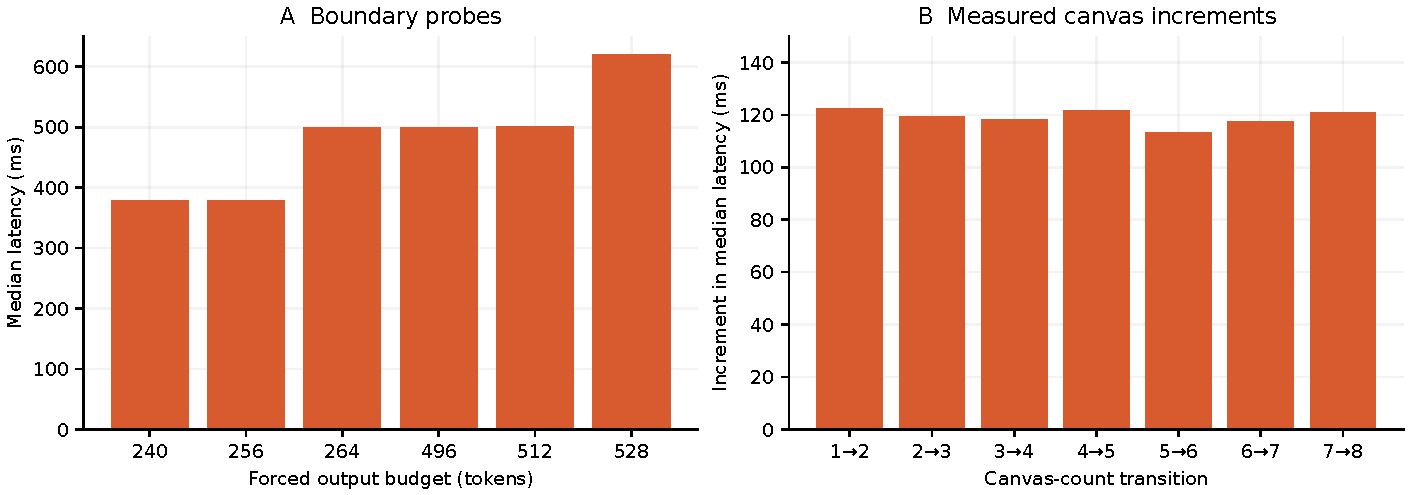
\includegraphics[width=\linewidth]{figures/fig2_canvas_edges.pdf}
\caption{DG canvas-boundary sweep ($K{=}8$, BGL, $n{=}200$ per cell).
Latency is approximately flat within each canvas and increases at the
boundary. The seven measured increments to $B{=}2048$ have median
\dgStep\,ms and range \dgStepLo--\dgStepHi\,ms. A constant
increment is a useful approximation within this sweep.}
\label{fig:edges}
\end{figure}

\subsection{Decoding effort and input dependence}
$K{=}8$ is a useful operating point in the tested quality--latency curve,
not a universal optimum. The $K$ sweep is nonlinear: measured latency
changes little from $K{=}8$ to $16$, then rises at $32$.
A line through the $K{=}2$ and $8$ observations gives an intercept near
143\,ms and a $K$-dependent contribution near 236\,ms at $K{=}8$.
This two-point interpolation does not identify prompt, attention, or
kernel costs, and cannot predict the benefit of a cache change
(Appendix~\ref{app:decomp}).

Longer prompts also increase latency. In the input-length experiment,
DG's fitted input slope is approximately \inputSlopeRatio$\times$
the dense AR-3B's. This is a secondary-model comparison, not an AR-30B
measurement. The dependence motivates the more general form
$T(L_{\mathrm{in}},N_C,K)$ and limits use of Eq.~\ref{eq:dg} when
schema width or conversational history changes
(Appendix~\ref{app:input_canvas}).

\paragraph{Transfer checks.}
At matched canvas size and $K$, the measured DG canvas increment changes
from \bglStep\,ms on BGL to \hdfsStep\,ms on the HDFS sample, a
1.7\% difference. This supports transfer of that increment between these
two settings. The AR slope comparison across corpora uses dense AR-3B.
For AR-30B, the HDFS median is \hdfsMedian\,ms (95\% bootstrap CI
[\hdfsCiLo, \hdfsCiHi]), with longer mean output than BGL; this
single operating point does not validate an entire cost curve.

HumanEval provides an exploratory task-transfer check
(Appendix~\ref{app:humaneval}). DG is faster in that harness but has
substantially lower pass@1 and syntax validity. Those measurements support
a latency--quality tradeoff, not a quality-matched code-generation speedup
or a demonstrated staircase across multiple code-output lengths.
